% !TeX root = ../main.tex
% -*- coding: utf-8 -*-

\chapter{基于近边界数据的模型所有权推断方法}\label{4}

尽管训练数据可以被公开,但用于推断模型所有权的数据需要私有化,否则攻击者就可以轻易地伪造近边界数据,无法成功推断模型所有权。因此本章通过生成对抗网络来对近边界数据进行特征学习,进而通过生成器生成新的、私有化的近边界数据。在此基础之上,使用私有化近边界数据微调源模型,使私有化近边界数据更靠近模型分类边界,数据越靠近分类边界,越有利于成功推断模型所有权。

结合上一章生成的初始近边界数据,本文方法的整体流程如图\ref{方法流程图}所示,主要包括三个阶段:(1)从公开数据集中生成近边界数据,(2)训练生成对抗模型生成新的、私有化的近边界数据,(3)使用私有化近边界数据微调源模型分类边界。

\begin{figure}[htbp]%%图,[htbp]是浮动格式
	\centering
	\setlength{\abovecaptionskip}{5mm} %图片标题与图片距离
%	\vspace{1mm}
%	\setlength{\belowcaptionskip}{-3mm} %调整图片标题与下文距离
	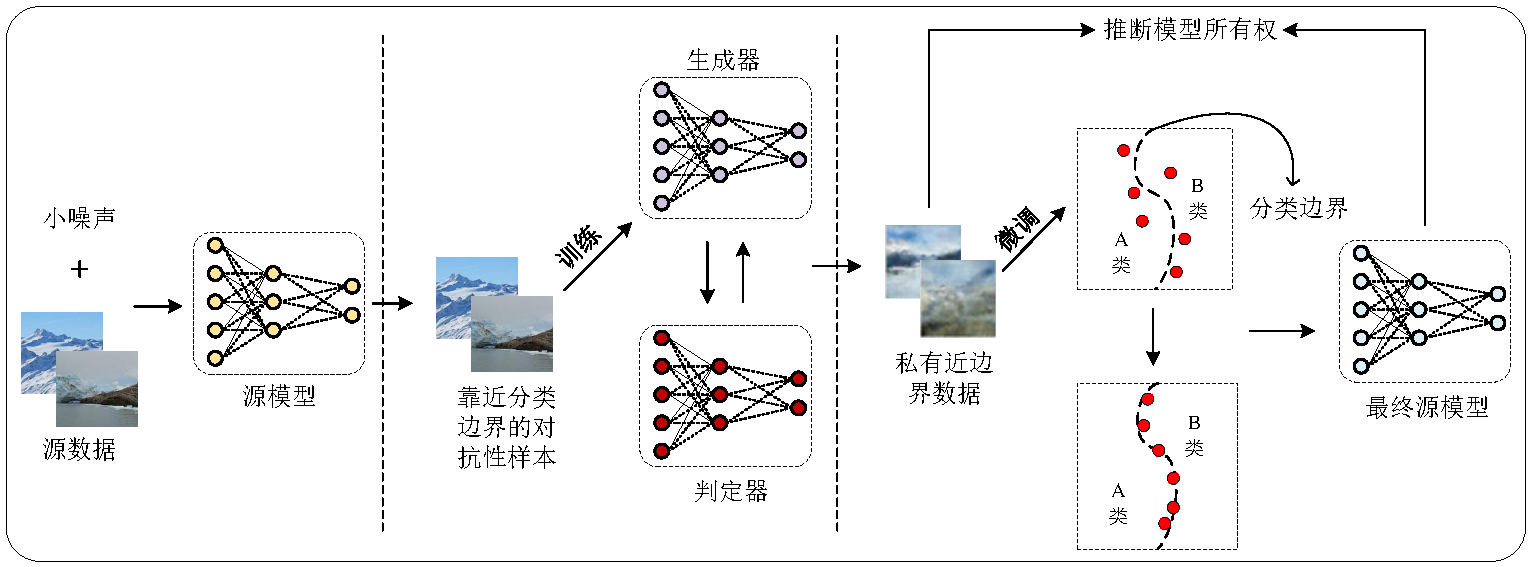
\includegraphics[width=1\linewidth]{方法流程图.pdf}
	\caption{方法流程图}
	\label{方法流程图}
	%	\vspace{-3mm}  %调整图片标题与下文距离,与\setlength{\belowcaptionskip}{-3mm}等效。
	\end {figure}



\section{近边界数据私有化}\label{4.1}

因为现在大多数模型训练使用的数据都来源于公开的数据集,所以通过生成对抗性样本的方法构建近边界数据这一步骤也十分容易复现。因此,本文需要从公开的训练数据中构建自己的私有化近边界数据,以防止模型所有者的近边界数据被轻易模仿。这是必要的步骤,因为近边界数据是后续推断模型所有权的核心依据。

本文希望可以通过训练一种模型学习上一节中生成的近边界对抗性样本的特征,并以此生成新的私有化近边界数据。这种新的数据从视觉上不一定和原始数据类似,但其原始的特征以及添加的噪声需要被学习,并根据提取到的特征生成的新样本对于源模型同样是近边界数据。

由\ref{2}\ref{2.3}可知,生成对抗网络在图像生成和特征提取方面有着显著的效果。本文考虑设计基于生成对抗网络的特征提取器,对初始近边界数据进行特征提取后,使用用生成器生成新的、私有化的近边界数据。

与生成初始近边界数据指标一致,本文需要寻找一种GAN,其生成的近边界数据到分类边界距离尽可能小。本文测试了几种常见的图像生成GAN,包括边界寻求生成对抗性网络(Boundary-Seeking Generative Adversarial Networks, BGAN)\cite{devon2017boundary},边界平衡生成对抗网络(Boundary Equilibrium Generative Adversarial Networks, BEGAN)\cite{berthelot2017began}和基于深度卷积生成对抗网络(Deep Convolutional Generative Adversarial Network, DCGAN)\cite{radford2015unsupervised}。大部分情况下,DCGAN的效果最好,具体的测试结果在\ref{5}\ref{5.3}中。因此,本文设计了一种基于DCGAN的特征提取器,提取近边界数据的特征之后,使用生成器生成私有化的近边界数据。
%注意生成器以,$CW$-$L_2$生成的对抗性示例作为输入,并输出私有化后的近边界数据。

\begin{figure}[htbp]%%图,[htbp]是浮动格式
	\centering
	\setlength{\abovecaptionskip}{5mm} %图片标题与图片距离
	%	\vspace{-2mm}
	\setlength{\belowcaptionskip}{-3mm} %调整图片标题与下文距离
	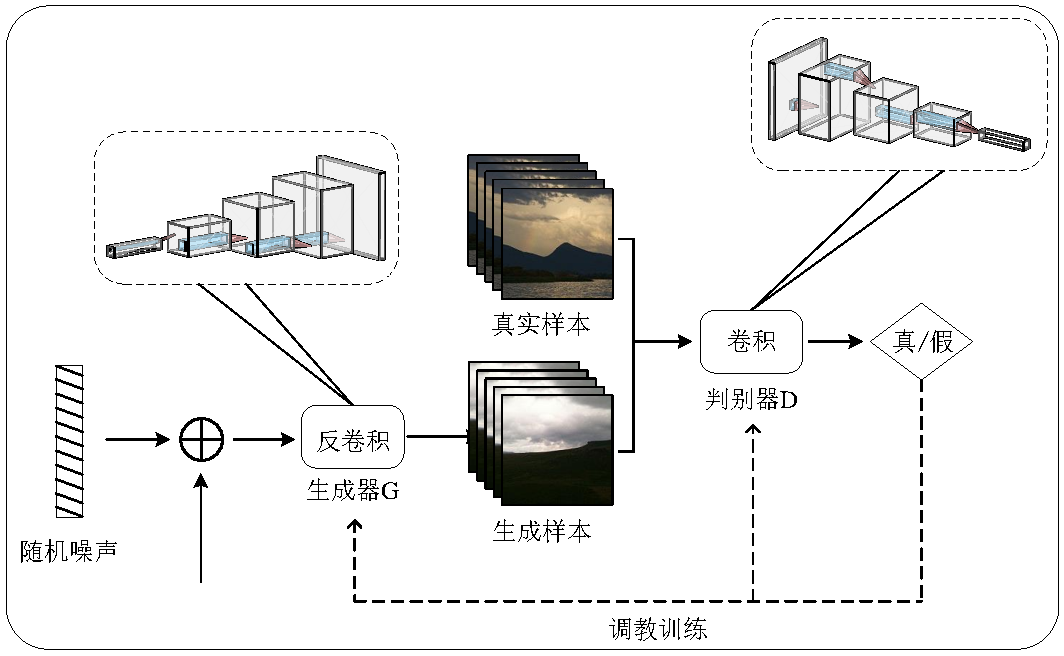
\includegraphics[width=1\linewidth]{DCGAN网络结构图.pdf}
	\caption{DCGAN网络结构图}
	\label{DCGAN网络结构图}
	%	\vspace{-3mm}  %调整图片标题与下文距离,与\setlength{\belowcaptionskip}{-3mm}等效。
	\end {figure}
	
如图\ref{DCGAN网络结构图}所示,DCGAN的大体结构与训练方式和普通GAN类似,主要变化是DCGAN将原始的GAN与CNN结合到一起,生成器$G$和判定器$D$都用CNN架构替换了原始GAN的全连接网络。得益于CNN对图像的强大处理能力,DCGAN极大提升了网络训练稳定性和生成样本的质量。具体而言,DCGAN主要是从网络架构上改进了原始的GAN,主要改进如下:

1)DCGAN的生成器和判别器均舍弃掉CNN的池化层,生成器使用反卷积层来还原图片,判别器保留CNN的整体架构,使用卷积层来提取图片特征。

2)在生成器和判别器中都使用Batch Normalization层,提升训练DCGAN模型稳定性的同时加速了训练。

3)生成器除最后一层使用Tanh激活函数外,其余层使用ReLU,判别器所有层均使用LeakyReLU,使模型可以更快的学习。

4)使用Adam优化器并调整了超参数,将学习率设置为0.0002,可以更好的学习到数据样本的特征。

本文需要DCGAN能够学习到尽可能多的近边界数据特征,以便更好的生成近边界数据。训练过程中,尝试修改DCGAN判定器的目标函数,在保留梯度的情况下,将其与源模型的结果相连,即使用源模型和判别器共同判定是生成数据还是原始数据。这种方式得到的训练结果在同样的生成规模下略微优于原始DCGAN生成的数据。然而,考虑到两者的效率,实际情况下生成的结果并无较大区别,所以本文采用原始的训练方式。训练DCGAN的具体流程如算法\ref{alg:2}所示。

\begin{algorithm}[!h] 
	\setstretch{1.2}
	\caption{\small 训练DCGAN模型}
	\label{alg:2}
	\small
	\begin{algorithmic}[1]
		\Require 近边界数据$\tilde{D}$;批处理大小$batchsize$;训练轮次$epoch$;损失函数$Loss$
		\Ensure 训练好的DCGAN模型
		\State 参数初始化:$learning \ rate \gets 0.0002$,$real\_label \gets 1$,$fake\_label \gets 0$
		\For{$i=1,2,...,epoch$}
		\State 随机噪声$z \gets 100$ 
		\State $x' \gets G(z)$
		\State $Loss1 \gets Loss(D(x), real\_label)$  \Comment $x$是近边界数据样本
		\State $Loss2 \gets Loss(D(x'), fake\_label)$
		\State $Loss_D \gets Loss1 + Loss2$
		\State $Loss_G \gets Loss(D(x'), real\_label)$ \Comment 生成器希望$D(x') $接近$real\_label$
		\State 使用Adam更新生成器$G$,判别器$D$的网络参数
		\EndFor
	\end{algorithmic}
	
\end{algorithm}

通过算法\ref{alg:2},完成训练DCGAN模型后,该模型可以被用作近边界数据特征提取器。通过生成器生成的图像,可以生成与初始近边界数据分布一致的私有近边界数据,这些数据仍然具备近边界性,并且可疑对手无法轻易获得。

在DCGAN的训练过程中,生成器和判定器相互博弈,以不断优化生成器生成图像的特征分布,使其逐渐接近原始近边界样本。训练收敛时,生成器已经学习到近边界数据的特征,因此可以生成新的私有近边界数据。

\section{源模型分类边界的微调}\label{4.2}

DCGAN对图像数据有着很强的特征提取能力,生成器能够很好的学习近边界数据特征,使用生成器构建的私有近边界数据仍然位于目标分类边界附近。但是相比于原始近边界数据,由于随机因素,生成的数据样本近边界性可能会弱于原始近边界数据,本文仍然希望近边界数据能最大程度上靠近目标分类边界。因为近边界数据与目标分类边界的距离越近,推断模型所有权成功的可能性就越大。此外,生成的私有近边界数据虽然只被模型所有者拥有,但对于一些功能易被泛化的模型,经过模型窃取攻击后,由于模型被修改,数据的近边界特性仍有可能被泛化。

因此,为了解决上述问题,本文提出使用近边界数据微调源模型的目标分类边界,使生成的私有近边界数据更加靠近DNN模型分类边界。如式\ref{eq:3.4}所示,$Loss_{FT}$是针对目标分类边界的损失函数。
\begin{equation}
	%	\setlength\abovedisplayshortskip{-3mm}
	\label{eq:3.9}
	Loss_{FT} = \frac{1}{n} \sum^{n}_{i = 1} (g_t(x_i') - g_s(x_i'))^2
\end{equation}

其中$n$是该目标分类边界的近边界数据的数量,$x_i'$是生成的近边界数据,$g_t(\cdot)$和$g_s(\cdot)$分别表示目标分类概率和源分类概率。

$Loss_{FT}$本质是希望近边界数据更靠近目标分类边界,但是为了尽可能减小对原始模型精度的影响,不能直接使用该损失函数对源模型进行微调。受DCGAN训练过程的启发,本文使用源模型的损失函数$Loss_{FM}$与$Loss_{FT}$两者交替训练微调源模型,并将学习率设置为0.0001,尽量减小源模型的变化幅度。本文希望在保持源模型精度的同时,使生成的数据样本更加靠近目标分类边界。与DCGAN的训练过程相似,微调源模型也是一个博弈的过程,微调的具体流程如算法\ref{alg:3}所示。

\begin{algorithm}[H] 
	\setstretch{1.2}
	\caption{\small 微调源模型}
	\label{alg:3}
	\small
	\begin{algorithmic}[1]
		\Require 原始数据集$D$;私有化近边界数据$D'$;批处理大小$batchsize$;训练轮次$epoch$;损失函数$Loss_{FT}$,$Loss_{FM}$;源模型$M$
		\Ensure 微调后的源模型$M'$
		\State 参数初始化:$learning \ rate \gets 0.0001$
		\For{$i=1,2,...,epoch$}                          
		\State $Loss1 \gets Loss_{FT}(g_t(x') , g_s(x'))$ \Comment $g_k(x')$:$x'$在第$k$类上的概率
		\State $Loss2 \gets Loss_{FM}(M(x), label)$ \Comment $label$指正常样本的原始标签
		\State 使用Adam更新源模型$M$的网络参数
		\EndFor
	\end{algorithmic}
	
\end{algorithm}

其中$x$指原始的数据样本,$x'$指DCGAN生成器生成的私有化近边界数据。

通过算法\ref{alg:3}微调目标分类边界使得私有近边界数据与源模型之间的联系更加紧密,这对后续能否成功推断模型所有权十分重要。在此算法中,本文只微调目标分类边界,且通过交替微调尽可能减少微调对源模型的影响。

\begin{table}[h]
	\centering
	%	\setlength{\arrayrulewidth}{0.5mm}
	\renewcommand\arraystretch{1.2}
	\caption{微调分类边界对模型的影响}
	\label{table:state}
	\small
	\begin{tabular*}{13cm}{@{\extracolsep{\fill}} l c c}
		
		
		
		\toprule[1pt]
		\textbf{数据集}        &    \textbf{微调前准确率}   &   \textbf{微调后准确率}            \\
		\hline
		CIFAR-10      &     0.886        &     0.873               \\
		
		Heritage      &     0.879        &     0.866               \\
		
		Intel\_image  &     0.854        &     0.846               \\
		\bottomrule[1pt]		
	\end{tabular*}
	
\end{table}

如表\ref{table:state}所示,正因为交替微调的设计和较小的学习率,源模型微调前后的精度差不超过3\%。因此,微调对于源模型的性能影响十分微小,甚至可以被忽略,但却有效提高了最后的所有权推断效果。更多微调目标分类边界对准确度的影响测试在\ref{5}\ref{5.4}中。

\section{推断可疑模型所有权}\label{4.3}

本文的方法适用于DNN分类模型的知识产权保护。一方面,该方法是利用近边界数据进行所有权推断,决策双方各自提供自己的近边界数据。将这些数据分别输入模型后,距离分类边界最近的数据提供者,获得模型的所有权,而不是进行类似模型水印和指纹的特定响应匹配,因此可以有效避免歧义攻击。另一方面,针对现有的数据集推断方法存在的问题,主要有以下两点改进:

1)本文在公开数据集上生成近边界数据代替私有训练数据,并且通过训练生成对抗网络生成新的、私有化的近边界数据,在解决数据集推断只能用于私有训练数据集问题的同时,也防止了本文的近边界数据被轻易复制和模仿,保持私有数据在推断模型所有权时的优势。

2)本文的方法利用近边界数据靠近决策边界的特性解决模型功能相似引起的误导。这是因为即使模型功能相似,但是决策边界不可能完全相同。如果近边界数据在可疑模型上并没有表现出近边界性,那么不会判定该模型是盗窃模型。\ref{5}\ref{5.4}中验证了这一点,本文提出的近边界数据,在无关模型上不会表现出近边界性。

\noindent\textbf{问题定义:}本文定义了一个DNN分类器$G$作为源模型,给定一个原始训练集$D$,假设该源模型是一个$n$-类的DNN分类器,分类器的输出层为softmax层或其他决策层,决策函数$g_j(x)$表示数据样本$x$被分到第$j$类的概率,其中$j$ = 1,2,..,$n$。$Z_1$,$Z_2$,..,$Z_n$表示模型分类器的全部决策函数输出,其结果可作为分类边界的依据被本文使用,因此

\begin{equation}
	g_j(x) = \frac{exp(Z_j(x))}{\sum_{i = 1}^n exp(Z_i(x))}
\end{equation}

\noindent 其中,数据样本$x$的标签$y$被推断拥有最大概率的类别,例如$y = arg \mathop{max} \limits_j g_j(x) = arg \mathop{max} \limits_j Z_j(x)$。

\subsection{设计目标}

根据现有的工作,本文提出的的方法在源模型训练后进行部署,且在黑盒环境下推断模型所有权。本文的方法不关注模型被盗窃的过程,而是聚焦在准确地推断DNN模型的所有权和识别不法分子的模型盗窃行为。现在大多数所有权验证技术都是基于黑盒环境。因为模型所有者和攻击者通常不会提供完整模型,而是以API的形式提供商业服务,因此黑盒模式的适用情况更加广泛。本文提出的方法仅利用模型提供的外部API,获取近边界数据的决策结果,从而推断模型所有权。

在通常的假设中,存在一个官方的仲裁机构,当对任一模型产生所有权怀疑时,受害者和可疑对手可以向机构提出申请并提供各自的私有化近边界数据,并通过本文的方法推断所有权。无论是在白盒的环境还是在黑盒的环境下,本文提出的方法均可以用来推断模型所有权。

本文提出的方法需要在面对各种盗窃模型时成功推断模型所有权,与此同时,需要保持DNN模型的性能并且不能对无关模型产生错误的所有权误导。因此本文提出方法的设计目标如下:

1)\textbf{精确性:}推断模型所有权的方法不应该影响模型的性能,模型的最大可接受测试精度下降不超过3\%。

2)\textbf{可继承性:}如果可疑模型与源模型相同或从源模型派生而来,则私有近边界数据在这些模型中均表现出近边界性。反之,近边界数据在无关模型中没有明显特征,防止产生所有权推断误导。

3)\textbf{有效性:}如果可疑模型与源模型相同或从源模型派生而来,则根据源模型构造的私有近边界数据比其他近边界数据更加靠近分类边界,这是本文方法成功推断模型所有权的依据。

4)\textbf{鲁棒性:}近边界数据应该对常见的模型修改(如模型微调、剪枝和有损压缩)具有鲁棒性,这是本文方法能广泛应用的关键。

5)\textbf{不可获得性:}敌手无法获得私有的近边界数据,否则私有近边界数据不在有更加靠近分类边界的优势,无法成功推断模型所有权。

6)\textbf{高效性:}通过近边界数据推断模型所有权应该能够高效地计算距离边界数据,并通过对比全部近边界数据的决策结果确定可疑模型是否是盗窃模型。

本文将在\ref{5}对该方法进行详细的实验评估,实验评估后,逐一验证分析是否达到这6个设计目标。

\subsection{方法概述}

本文提出了近边界数据,一种分布在分类边界附近的特殊样本。模型指纹使用对抗性样本抽象地反映模型分类边界,同一组对抗性样本的输入,其引起的决策模式的变化可以用于比较模型知识的相似性,但这种方法是脆弱的,一般的模型窃取攻击都会修改源模型,而对模型的任意修改操作都有可能破坏这种特性。因此,本文不直接比较决策模式的变化,它是不可信任的,而是比较对抗性样本与决策边界的距离。大多数对抗性样本都是位于决策边界附近的,也就是说,它们与决策边界的距离很近。对抗性样本的这种性质被本文所利用并构造近边界数据,经过测试,本文发现绝大多数的模型窃取方法都无法改变这种结果,即使样本分类被影响,其仍然位于分类边界附近。

近边界数据背后的意义是数据的近边界特性不会因为受到模型窃取攻击产生的模型修改而消失。受到这个特点的启发,将近边界数据作为水印验证所有权是传统的思路,虽然不会对模型的精度造成影响,但是这样的水印是脆弱的,很容易受到御歧义攻击,因此本文提出由近边界数据驱动的所有权推断方法。
%\begin{figure}[htb]%%图,[htbp]是浮动格式
%	\centering
%	\setlength{\abovecaptionskip}{5mm} %图片标题与图片距离
%	%	\vspace{-2mm}
%	\setlength{\belowcaptionskip}{-3mm} %调整图片标题与下文距离
%	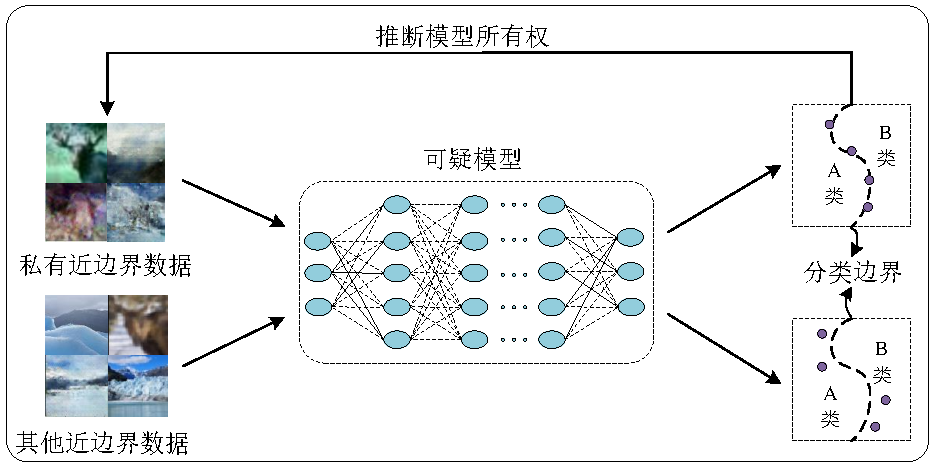
\includegraphics[width=1\linewidth]{方法原理图.pdf}
%	\caption{近边界数据推断所有权}
%	\label{方法原理图}
%	%	\vspace{-3mm}  %调整图片标题与下文距离,与\setlength{\belowcaptionskip}{-3mm}等效。
%	\end {figure}

\begin{figure}[htbp]%%图,[htbp]是浮动格式
	\centering
	\setlength{\abovecaptionskip}{5mm} %图片标题与图片距离
	%	\vspace{-2mm}
%	\setlength{\belowcaptionskip}{-3mm} %调整图片标题与下文距离
	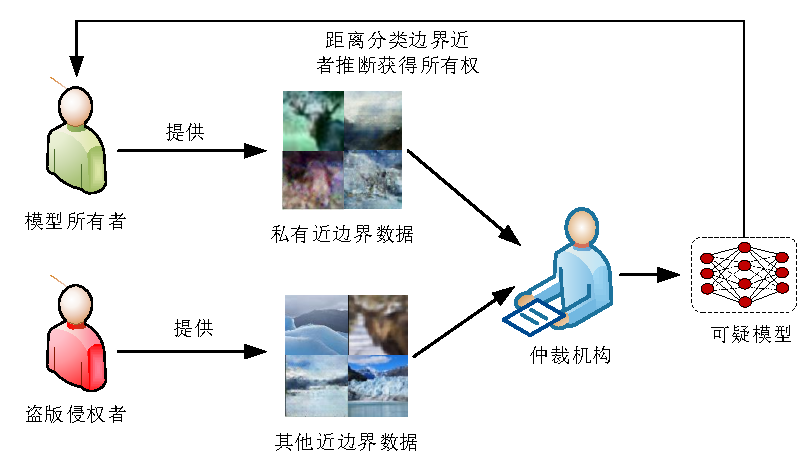
\includegraphics[width=0.8\linewidth]{推断示意图.pdf}
	\caption{推断示意图}
	\label{推断示意图}
	%	\vspace{-3mm}  %调整图片标题与下文距离,与\setlength{\belowcaptionskip}{-3mm}等效。
	\end {figure}

如图\ref{推断示意图}所示,本文提出方法的主要思想是构造私有的近边界数据,以数据驱动推断模型的所有权。当模型所有者怀疑可疑模型是盗窃自己的模型时,向官方机构发起仲裁。模型所有者和可疑对手分别提供各自的私有近边界数据,仲裁机构分别计算双方数据的输出结果,统计测试样本数据点到分类边界的距离,距离近的判定获得模型所有权。


\subsection{假设检验}\label{3.3.3}

根据\ref{3}的讨论结果,本文认为过去的验证模型所有权的思路具有较大的局限性,大多数研究无法抵御歧义攻击。因此,本文提出了推断模型所有权的方法,这是一种“最”的思路。与过去工作中利用模型水印和指纹验证模型所有权相比,本文方法使用数据在对应模型上结果作为所有权推断依据,结果的可比性和唯一性可以有效避免歧义攻击。

上一小节中提到,模型所有者向仲裁机构提出仲裁并提供近边界数据,盗窃者同样需要提供相应的近边界数据,仲裁机构分别计算各自数据到目标分类边界距离,最靠近目标分类边界的近边界数据所有者将获得模型所有权。由于近边界数据通常是一组数据,所以应该根据统计的结果来看。在实验中,本文计算了不同规模的近边界数据组在源模型、盗窃模型以及不相关模型上到分类边界的距离,并设计了一种基于假设检验的方法来表现推断的置信度。

\noindent\textbf{假设检验:}本文假设事件$C$是模型所有者提供的私有近边界数据在可疑模型上的计算结果,事件$C_S$ 表示盗窃者提供的近边界数据在可疑模型上的计算结果,或模型所有者提供的私有近边界数据在无关模型上的计算结果。本文计算假设$H_0:\mu \geq \mu_S(H_1:\mu < \mu_S)$的$p$值,以及差异大小$\Delta \mu = \mu_S - \mu$,$\Delta\mu$越大,推断可信度越高。如果$p$值低于预定义的置信度评分$\alpha$,则拒绝$H_0$,并称正在测试的模型是被盗模型。本文重复30次统计性实验以提高可信度,假设检验的具体过程如算法\ref{alg:4}所示。

\begin{algorithm}[H] 
	\setstretch{1.2}
	\caption{\small 假设检验}
	\label{alg:4}
	\small
	\begin{algorithmic}[1]
		\Require 模型所有者私有近边界数据样本$X$;可疑对手近边界数据样本$X_S$;可疑模型$\tilde{M}$;假设检验对照表$T$;显著性水平$\alpha$
		\Ensure 可疑模型是否为盗窃模型
		\State 原假设:$H_0:\mu \geq \mu_S$
		\State 备择假设:$H_1:\mu < \mu_S$
		\State 计算模型所有者私有近边界数据样本均值$\overline{X}$                     
		\State 计算可疑对手近边界数据样本均值$\overline{X}_S$ 
		\State 计算统计量$t$
		\State 查对照表$T$获得临界值$\lambda$
		\If{$t > \lambda$}
		\State $p < \alpha$,拒绝$H_0$,接受$H_1$,可疑模型是被盗模型
		\Else \State $p > \alpha$,不拒绝$H_0$
		\EndIf
	\end{algorithmic}
\end{algorithm}

结合生成使用CW-$L_2$生成初始近边界数据和使用DCGAN私有化近边界数据的过程,加上假设检验比对结果的差异性,本文提出方法的整体执行流程如图\ref{方法整体流程图}所示。



\section{本章小结}

近边界数据是本文方法推断所有权的依据,不能轻易被盗窃者复制伪造。本章使用初始近边界数据训练DCGAN,使之学习到近边界数据的特征,然后使用生成器生成新的、私有化的近边界数据,使所有者保持私有数据的优势。接着设计了新的损失函数并微调源模型,使近边界数据更加靠近目标分类边界,增强本文方法面对各种模型盗窃技术的性能和防御性。然后在私有近边界数据的基础上,提出本文基于近边界数据的模型所有权推断方法,最后提出使用假设检验的方法来比对推测结果的差异性。

\begin{figure}[htb]%%图,[htbp]是浮动格式
	\centering
	\setlength{\abovecaptionskip}{5mm} %图片标题与图片距离
	%		\vspace{-2mm}
	%	\setlength{\belowcaptionskip}{-3mm} %调整图片标题与下文距离
	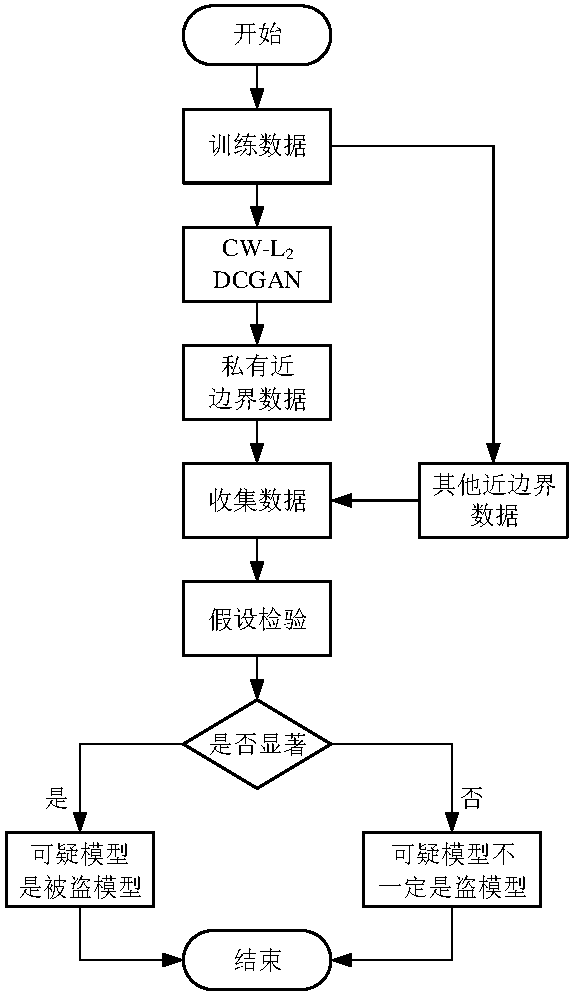
\includegraphics[width=0.50\linewidth]{方法整体流程图.pdf}
	\caption{方法整体流程图}
	\label{方法整体流程图}
	%	\vspace{-3mm}  %调整图片标题与下文距离,与\setlength{\belowcaptionskip}{-3mm}等效。
	\end {figure}